\chapter{Conception Détaillée}

L’application mobile est codée en React Native qui est une bibliothèque de JavaScript. L’application communique avec l’API pour tout ce qui est donnée de l’utilisateur (le nom d’utilisateur, le mot de passe, ces trajets, ces localisations …). L’application en elle-même est composé de deux parties : la partie de login et le contenu de l’application

Petit point sur React Native :

React native est React mais pour les applications mobiles. Ce langage est un peu particulier car c’est plutôt un langage fonctionnel. Un composant en react est une classe qui hérite de React et suis ce cycle de vie d’après la documentation officiel de React  :
“Phase de Render” : Méthodes pures, sans effets secondaires. Peuvent être interrompues, annulées ou redémarrées par React.
“Phase de Commit” : Peuvent opérer sur le DOM, engendrer des effets secondaires, programmer des mises à jour.
Plus d’information sur le cycle de vie d’un composant ici :

https://projects.wojtekmaj.pl/react-lifecycle-methods-diagram/

Et pour React ici :

https://fr.reactjs.org/


Nous allons expliquer le fonctionnement de chaque composant :

\section{App.js}

En React native l’application charge le composant App.js au lancement de l’application. Dans ce composant on y retrouve principalement un appel à d’autre composants (dans notre cas MesComposants) pour ne pas écrire tout le code dans un seul et même ficher. Nous y retrouvons aussi une déclaration de store et des reducers du module redux. Ce module permet la communication entre tous les composants de notre application (ce qui n’ai pas possible sans ce module en react ) . Tous les composants sont connectés au « magasin » et peuvent modifier ou accéder à ces valeurs

\section{MesComposant.js}

Ce composant sert juste de composant intermédiaire, il affiche le contenue de l’application quand un utilisateur se connecter sinon il affiche la page de connexion.

Code :

Le rendu se fait en fonction d’une variable booléenne dans le magasin et qui change quand l’utilisateur se connecte ou se déconnecte

\section{ContenuPageLogin.js}

Ce composant affiche PageLogin et crée un drawer entre PageLogin et PageCreationdeCompte (un drawer permet la navigation d’une page a une autre)

\section{PageLogin.js}

Ce composant sert à se connecter à notre API, il affiche une erreur si les identifiants utilisé sont incorrects (grâce à une petite popup) et redirige vers le composant PageCreationdeCompte quand l’utilisateur clique sur ce crée un compte

Code :

Les variables du nom d’utilisateur et de mot de passe sont actualisé à chaque changement dans les champs texte
Quand on clique sur le bouton login, sa lance une fonction qui fait un requête http à l’API et si tout se passe bien (bon login/password), il y a un changement de la variable dans le magasin qui gère la connexion sinon cela affiche un message d’erreur

\section{PageCreationdeCompte}

Ce n’ai pas un ficher javascript mais une fonction, en effet en react un composant peut prendre la forme d’une classe qui hérite de React , ou une fonction qui retourne du React. Dans ce composant nous affichons un site web qui permet de se crée un compte pour notre application.

Code :

Une simple utilisation d’une Webview

\section{ContenuApp.js}

C’est dans ce composant que l’application utile est. On y retrouve la création d’une navigation par onglet en bas de l’écran. Chaque onglet représente un composant Map, Statistique et options et on y navigue en cliquant dessus.

Code :

On crée une barre de navigation en bas de l’écran et on lui fournit un composant un nom et des options (comme des images)
On crée aussi un Stack de navigation pour la navigation entre Stats et DetailTrajet

\section{Map.js}

Ce composant sert à afficher la carte. Sur cette carte on y retrouve la position actuelle de l’utilisateur, la position du Ghost si une course est lancée.
La position de l’utilisateur est actualisée chaque fois qu’il bouge, de même pour le Ghost.
Il y a aussi une gestion d’envoie des positions à l’API lorsque l’utilisateur enregistre un trajet (qu’il peut activer dans le composant detailTrajet que nous verrons juste après).

Code :

On regarde à chaque changement de positions plusieurs variable : les variables dans les magasins qui nous informe si un trajet est en cours ou si une course est en cours. Si une course est en cours nous avons la liste de ce des positions de ce trajet dans le magasin et nous actualisons la position du fantôme sur la carte a chaque changement de position de l’utilisateur. Si le Ghost arrive en premier une popup apparait et change l’état dans le magasin.
Même logique pour les trajets.

\section{Stats.js}
C’est ici que l’utilisateur peut voir tous ces catégories qu’il a déjà enregistrées, il peut aussi en crée.
Toute ces catégories sont changées au rendu du composant depuis l’API.
Un appuie simple permet de naviguer au composant detailTrajet et un appuie long permet de supprimer la catégorie voulue de l’API.

Code :

Au montage premier montage du composant nous récupérons toutes les catégories et les affichons, l’ajout de catégories par le bouton change l’état du composant ce qui trigger un nouveau rendu de l’affichage.

\section{DetailTrajet.js}
Ce composant permet d’afficher tous les trajets d’une catégorie (qui sont toujours récupérer de l’API). Appuyer sur un trajet ouvre laisse plusieurs choix à l’utilisateur :

Rien : la popup disparait

Supprimer : Supprimer le trajet voulu

Faire une course de ce trajet : L’application va charger le trajet et quand cette opération est finie on navigue directement vers la carte avec le Ghost prêt à la course. Propose aussi de crée un nouveau trajet ( pas obligatoire)

Affiche les statistiques : Affiche un overlay avec les statistiques du trajet voulu sur le site GhostRun

Nous avons aussi deux boutons pour commencer un trajet et en finir un, pour commencer un trajet l’utilisateur doit choisir juste un mode de transport parmi ceux qui sont proposé.

Code :

Même logique que les catégories (avec un affichage différent).
Quand la liste des positions d’un trajet pour faire une course a fini d’être récupère, nous naviguons vers la carte mais avec un paramètre en plus qui est cette liste.

\section{Option.js}

Dans ce composant l’utilisateur peut se déconnecter et revenir a la page de connexion, ou bien passer au thème sombre sur la carte.

Code :

Le bouton de déconnection change la variable dans le magasin du fait d’être connecter ou non, et le switch change juste la variable de style de la carte

\section{Architecture de l'application}

\begin{figure}[h]
    \centering
    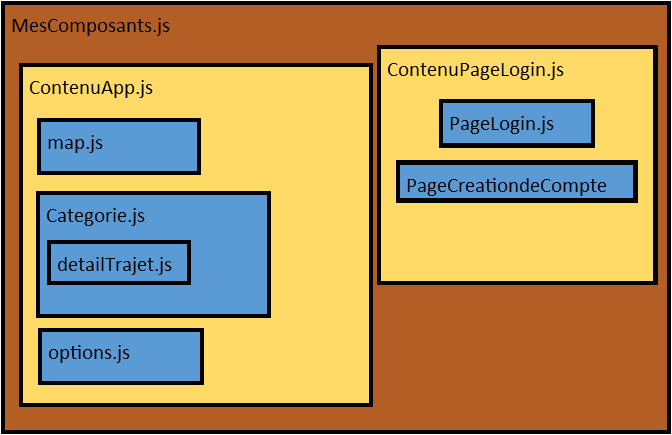
\includegraphics[keepaspectratio, width=2\textwidth/2, height=2\textheight/5]{ima/archticture.png}
    \caption{Archticture de l'application mobile }
    \label{fig:25-archticture}
\end{figure}




